\section{Defining a final class}\label{defining-a-final-class}

\subsection{A very simple editor}\label{a-very-simple-editor}

We made a very simple file viewer in the previous section. Now we go on
to rewrite it and turn it into very simple editor. Its source file is
\passthrough{\lstinline!tfe1.c!} (text file editor 1) under
\passthrough{\lstinline!tfe!} directory.

GtkTextView is a multi-line editor. So, we don't need to write the
editor from scratch. We just add two things to the file viewer:

\begin{itemize}
\tightlist
\item
  Pointers to GFile instances.
\item
  A text-save function.
\end{itemize}

There are a couple of ways to store the pointers.

\begin{itemize}
\tightlist
\item
  Use global variables
\item
  Make a child class of GtkTextView and its each instance holds a
  pointer to the GFile instance.
\end{itemize}

Using global variables is easy to implement. Define a sufficient size
pointer array to GFile. For example,

\begin{lstlisting}[language=C]
GFile *f[20];
\end{lstlisting}

The variable \passthrough{\lstinline!f[i]!} corresponds to the file
associated with the i-th GtkNotebookPage.

However, There are two problems. The first is the size of the array. If
a user gives too many arguments (more than 20 in the example above), it
is impossible to store all the pointers to the GFile instances. The
second is difficulty to maintain the program. We have a small program so
far. But, the more you develop the program, the bigger its size grows.
Generally speaking, it is very difficult to maintain global variables in
a big program. When you check the global variable, you need to check all
the codes that use the variable.

Making a child class is a good idea in terms of maintenance. And we
prefer it rather than a global variable.

Be careful that we are thinking about ``child class'', not ``child
widget''. Child class and child widget are totally different. Class is a
term of GObject system. If you are not familiar with GObject, see:

\begin{itemize}
\tightlist
\item
  \href{https://docs.gtk.org/gobject/}{GObject API reference}
\item
  \href{https://toshiocp.github.io/Gobject-tutorial/}{GObject tutorial
  for beginners}
\end{itemize}

A child class inherits everything from the parent and, in addition,
extends its performance. We will define TfeTextView as a child class of
GtkTextView. It has everything that GtkTextView has and adds a pointer
to a GFile.

\begin{figure}
\centering
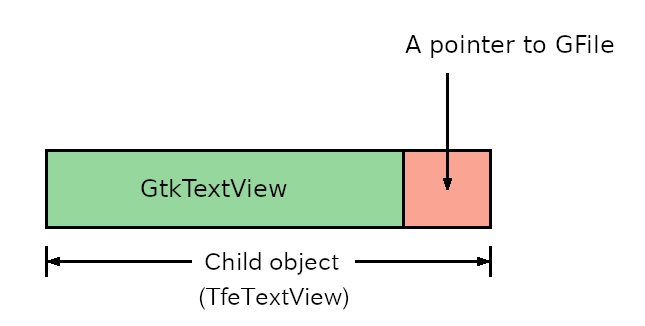
\includegraphics[width=9.675cm,height=4.89cm]{../image/child.png}
\caption{Child object of GtkTextView}
\end{figure}

\subsection{How to define a child class of
GtkTextView}\label{how-to-define-a-child-class-of-gtktextview}

You need to know GObject system convention. First, look at the program
below.

\begin{lstlisting}[language=C]
#define TFE_TYPE_TEXT_VIEW tfe_text_view_get_type ()
G_DECLARE_FINAL_TYPE (TfeTextView, tfe_text_view, TFE, TEXT_VIEW, GtkTextView)

struct _TfeTextView
{
  GtkTextView parent;
  GFile *file;
};

G_DEFINE_FINAL_TYPE (TfeTextView, tfe_text_view, GTK_TYPE_TEXT_VIEW);

static void
tfe_text_view_init (TfeTextView *tv) {
}

static void
tfe_text_view_class_init (TfeTextViewClass *class) {
}

void
tfe_text_view_set_file (TfeTextView *tv, GFile *f) {
  tv -> file = f;
}

GFile *
tfe_text_view_get_file (TfeTextView *tv) {
  return tv -> file;
}

GtkWidget *
tfe_text_view_new (void) {
  return GTK_WIDGET (g_object_new (TFE_TYPE_TEXT_VIEW, NULL));
}
\end{lstlisting}

\begin{itemize}
\tightlist
\item
  TfeTextView is divided into two parts. Tfe and TextView. Tfe is called
  prefix or namespace. TextView is called object.
\item
  There are three different identifier patterns. TfeTextView (camel
  case), tfe\_text\_view (this is used for functions) and
  TFE\_TEXT\_VIEW (This is used to cast a object to TfeTextView).
\item
  First, define \passthrough{\lstinline!TFE\_TYPE\_TEXT\_VIEW!} macro as
  \passthrough{\lstinline!tfe\_text\_view\_get\_type ()!}. The name is
  always (prefix)\_TYPE\_(object) and the letters are upper case. And
  the replacement text is always (prefix)\_(object)\_get\_type () and
  the letters are lower case. This definition is put before
  \passthrough{\lstinline!G\_DECLARE\_FINAL\_TYPE!} macro.
\item
  The arguments of \passthrough{\lstinline!G\_DECLARE\_FINAL\_TYPE!}
  macro are the child class name in camel case, lower case with
  underscore, prefix (upper case), object (upper case with underscore)
  and parent class name (camel case). The following two C structures are
  declared in the expansion of the macro.

  \begin{itemize}
  \tightlist
  \item
    \passthrough{\lstinline!typedef struct \_TfeTextView TfeTextView!}
  \item
    \passthrough{\lstinline!typedef struct \{GtkTextViewClass parent\_class; \} TfeTextViewClass;!}
  \end{itemize}
\item
  These declaration tells us that TfeTextView and TfeTextViewClass are C
  structures. ``TfeTextView'' has two meanings, class name and C
  structure name. The C structure TfeTextView is called object.
  Similarly, TfeTextViewClass is called class.
\item
  Declare the structure \passthrough{\lstinline!\_TfeTextView!}. The
  underscore is necessary. The first member is the parent object (C
  structure). Notice this is not a pointer but the object itself. The
  second member and after are members of the child object. TfeTextView
  structure has a pointer to a GFile instance as a member.
\item
  \passthrough{\lstinline!G\_DEFINE\_FINEL\_TYPE!} macro. The arguments
  are the child object name in camel case, lower case with underscore
  and parent object type (prefix)\_TYPE\_(module). This macro is mainly
  used to register the new class to the type system. Type system is a
  base system of GObject. Every class has its own type. The types of
  GObject, GtkWidget and TfeTextView are
  \passthrough{\lstinline!G\_TYPE\_OBJECT!},
  \passthrough{\lstinline!GTK\_TYPE\_WIDGET!} and
  \passthrough{\lstinline!TFE\_TYPE\_TEXT\_VIEW!} respectively. For
  example, \passthrough{\lstinline!TFE\_TYPE\_TEXT\_VIEW!} is a macro
  and it is expanded to a function
  \passthrough{\lstinline!tfe\_text\_view\_get\_type()!}. It returns a
  integer which is unique among all GObject system classes.
\item
  The instance init function
  \passthrough{\lstinline!tfe\_text\_view\_init!} is called when the
  instance is created. It is the same as a constructor in other object
  oriented languages.
\item
  The class init function
  \passthrough{\lstinline!tfe\_text\_view\_class\_init!} is called when
  the class is created.
\item
  Two functions \passthrough{\lstinline!tfe\_text\_view\_set\_file!} and
  \passthrough{\lstinline!tfe\_text\_view\_get\_file!} are public
  functions. Public functions are open and you can call them anywhere.
  They are the same as public method in other object oriented languages.
  \passthrough{\lstinline!tv!} is a pointer to the TfeTextView object (C
  structure). It has a member \passthrough{\lstinline!file!} and it is
  pointed by \passthrough{\lstinline!tv->file!}.
\item
  TfeTextView instance creation function is
  \passthrough{\lstinline!tfe\_text\_view\_new!}. Its name is
  (prefix)\_(object)\_new. It uses
  \passthrough{\lstinline!g\_object\_new!} function to create the
  instance. The arguments are (prefix)\_TYPE\_(object), a list to
  initialize properties and NULL. NULL is the end mark of the property
  list. No property is initialized here. And the return value is casted
  to GtkWidget.
\end{itemize}

This program shows the outline how to define a child class.

\subsection{Close-request signal}\label{close-request-signal}

Imagine that you are using this editor. First, you run the editor with
arguments. The arguments are filenames. The editor reads the files and
shows the window with the text of files in it. Then you edit the text.
After you finish editing, you click on the close button of the window
and quit the editor. The editor updates files just before the window
closes.

GtkWindow emits the ``close-request'' signal when the close button is
clicked. We will connect the signal and the handler
\passthrough{\lstinline!before\_close!}. (A handler is a C function
which is connected to a signal.) The function
\passthrough{\lstinline!before\_close!} is called when the signal
``close-request'' is emitted.

\begin{lstlisting}[language=C]
g_signal_connect (win, "close-request", G_CALLBACK (before_close), NULL);
\end{lstlisting}

The argument \passthrough{\lstinline!win!} is a GtkApplicationWindow, in
which the signal ``close-request'' is defined, and
\passthrough{\lstinline!before\_close!} is the handler. The
\passthrough{\lstinline!G\_CALLBACK!} cast is necessary for the handler.
The program of \passthrough{\lstinline!before\_close!} is as follows.

\begin{lstlisting}[language=C, numbers=left]
static gboolean
before_close (GtkWindow *win, GtkWidget *nb) {
  GtkWidget *scr;
  GtkWidget *tv;
  GFile *file;
  char *pathname;
  GtkTextBuffer *tb;
  GtkTextIter start_iter;
  GtkTextIter end_iter;
  char *contents;
  unsigned int n;
  unsigned int i;
  GError *err = NULL;

  n = gtk_notebook_get_n_pages (GTK_NOTEBOOK (nb));
  for (i = 0; i < n; ++i) {
    scr = gtk_notebook_get_nth_page (GTK_NOTEBOOK (nb), i);
    tv = gtk_scrolled_window_get_child (GTK_SCROLLED_WINDOW (scr));
    file = tfe_text_view_get_file (TFE_TEXT_VIEW (tv));
    tb = gtk_text_view_get_buffer (GTK_TEXT_VIEW (tv));
    gtk_text_buffer_get_bounds (tb, &start_iter, &end_iter);
    contents = gtk_text_buffer_get_text (tb, &start_iter, &end_iter, FALSE);
    if (! g_file_replace_contents (file, contents, strlen (contents), NULL, TRUE, G_FILE_CREATE_NONE, NULL, NULL, &err)) {
      g_printerr ("%s.\n", err->message);
      g_clear_error (&err);
    }
    g_free (contents);
    g_object_unref (file);
  }
  return FALSE;
}
\end{lstlisting}

The numbers on the left are line numbers.

\begin{itemize}
\tightlist
\item
  15: The number of note book pages is assigned to
  \passthrough{\lstinline!n!}.
\item
  16-29: For loop with regard to the index to each page.
\item
  17-19: \passthrough{\lstinline!scr!}, \passthrough{\lstinline!tv!} and
  \passthrough{\lstinline!file!} is assigned pointers to the
  GtkScrolledWindow, TfeTextView and GFile. The GFile of TfeTextView was
  stored when \passthrough{\lstinline!app\_open!} handler was called. It
  will be shown later.
\item
  20-22: \passthrough{\lstinline!tb!} is assigned the GtkTextBuffer of
  the TfeTextView. The contents of the buffer are accessed with
  iterators. Iterators points somewhere in the buffer. The function
  \passthrough{\lstinline!gtk\_text\_buffer\_get\_bounds!} assigns the
  start and end of the buffer to \passthrough{\lstinline!start\_iter!}
  and \passthrough{\lstinline!end\_iter!} respectively. Then the
  function \passthrough{\lstinline!gtk\_text\_buffer\_get\_text!}
  returns the text between \passthrough{\lstinline!start\_iter!} and
  \passthrough{\lstinline!end\_iter!}, which is the whole text in the
  buffer.
\item
  23-26: The text is saved to the file. If it fails, error messages are
  displayed. The GError instance must be freed and the pointer
  \passthrough{\lstinline!err!} needs to be NULL for the next run in the
  loop.
\item
  27: \passthrough{\lstinline!contents!} are freed.
\item
  28: GFile is useless. \passthrough{\lstinline!g\_object\_unref!}
  decreases the reference count of the GFile. Reference count will be
  explained in the later section. The reference count will be zero and
  the GFile instance will destroy itself.
\end{itemize}

\subsection{Source code of tfe1.c}\label{source-code-of-tfe1.c}

The following is the whole source code of
\passthrough{\lstinline!tfe1.c!}.

\begin{lstlisting}[language=C, numbers=left]
#include <gtk/gtk.h>

/* Define TfeTextView Widget which is the child class of GtkTextView */

#define TFE_TYPE_TEXT_VIEW tfe_text_view_get_type ()
G_DECLARE_FINAL_TYPE (TfeTextView, tfe_text_view, TFE, TEXT_VIEW, GtkTextView)

struct _TfeTextView
{
  GtkTextView parent;
  GFile *file;
};

G_DEFINE_FINAL_TYPE (TfeTextView, tfe_text_view, GTK_TYPE_TEXT_VIEW);

static void
tfe_text_view_init (TfeTextView *tv) {
  tv->file = NULL;
}

static void
tfe_text_view_class_init (TfeTextViewClass *class) {
}

void
tfe_text_view_set_file (TfeTextView *tv, GFile *f) {
  tv->file = f;
}

GFile *
tfe_text_view_get_file (TfeTextView *tv) {
  return tv -> file;
}

GtkWidget *
tfe_text_view_new (void) {
  return GTK_WIDGET (g_object_new (TFE_TYPE_TEXT_VIEW, NULL));
}

/* ---------- end of the definition of TfeTextView ---------- */

static gboolean
before_close (GtkWindow *win, GtkWidget *nb) {
  GtkWidget *scr;
  GtkWidget *tv;
  GFile *file;
  char *pathname;
  GtkTextBuffer *tb;
  GtkTextIter start_iter;
  GtkTextIter end_iter;
  char *contents;
  unsigned int n;
  unsigned int i;
  GError *err = NULL;

  n = gtk_notebook_get_n_pages (GTK_NOTEBOOK (nb));
  for (i = 0; i < n; ++i) {
    scr = gtk_notebook_get_nth_page (GTK_NOTEBOOK (nb), i);
    tv = gtk_scrolled_window_get_child (GTK_SCROLLED_WINDOW (scr));
    file = tfe_text_view_get_file (TFE_TEXT_VIEW (tv));
    tb = gtk_text_view_get_buffer (GTK_TEXT_VIEW (tv));
    gtk_text_buffer_get_bounds (tb, &start_iter, &end_iter);
    contents = gtk_text_buffer_get_text (tb, &start_iter, &end_iter, FALSE);
    if (! g_file_replace_contents (file, contents, strlen (contents), NULL, TRUE, G_FILE_CREATE_NONE, NULL, NULL, &err)) {
      g_printerr ("%s.\n", err->message);
      g_clear_error (&err);
    }
    g_free (contents);
    g_object_unref (file);
  }
  return FALSE;
}

static void
app_activate (GApplication *app) {
  g_print ("You need to give filenames as arguments.\n");
}

static void
app_open (GApplication *app, GFile ** files, gint n_files, gchar *hint) {
  GtkWidget *win;
  GtkWidget *nb;
  GtkWidget *lab;
  GtkNotebookPage *nbp;
  GtkWidget *scr;
  GtkWidget *tv;
  GtkTextBuffer *tb;
  char *contents;
  gsize length;
  char *filename;
  int i;
  GError *err = NULL;

  win = gtk_application_window_new (GTK_APPLICATION (app));
  gtk_window_set_title (GTK_WINDOW (win), "file editor");
  gtk_window_set_default_size (GTK_WINDOW (win), 600, 400);

  nb = gtk_notebook_new ();
  gtk_window_set_child (GTK_WINDOW (win), nb);

  for (i = 0; i < n_files; i++) {
    if (g_file_load_contents (files[i], NULL, &contents, &length, NULL, &err)) {
      scr = gtk_scrolled_window_new ();
      tv = tfe_text_view_new ();
      tb = gtk_text_view_get_buffer (GTK_TEXT_VIEW (tv));
      gtk_text_view_set_wrap_mode (GTK_TEXT_VIEW (tv), GTK_WRAP_WORD_CHAR);
      gtk_scrolled_window_set_child (GTK_SCROLLED_WINDOW (scr), tv);

      tfe_text_view_set_file (TFE_TEXT_VIEW (tv),  g_file_dup (files[i]));
      gtk_text_buffer_set_text (tb, contents, length);
      g_free (contents);
      filename = g_file_get_basename (files[i]);
      lab = gtk_label_new (filename);
      gtk_notebook_append_page (GTK_NOTEBOOK (nb), scr, lab);
      nbp = gtk_notebook_get_page (GTK_NOTEBOOK (nb), scr);
      g_object_set (nbp, "tab-expand", TRUE, NULL);
      g_free (filename);
    } else {
      g_printerr ("%s.\n", err->message);
      g_clear_error (&err);
    }
  }
  if (gtk_notebook_get_n_pages (GTK_NOTEBOOK (nb)) > 0) {
    g_signal_connect (win, "close-request", G_CALLBACK (before_close), nb);
    gtk_window_present (GTK_WINDOW (win));
  } else
    gtk_window_destroy (GTK_WINDOW (win));
}

int
main (int argc, char **argv) {
  GtkApplication *app;
  int stat;

  app = gtk_application_new ("com.github.ToshioCP.tfe1", G_APPLICATION_HANDLES_OPEN);
  g_signal_connect (app, "activate", G_CALLBACK (app_activate), NULL);
  g_signal_connect (app, "open", G_CALLBACK (app_open), NULL);
  stat =g_application_run (G_APPLICATION (app), argc, argv);
  g_object_unref (app);
  return stat;
}
\end{lstlisting}

\begin{itemize}
\tightlist
\item
  109: The GFile pointer of the TfeTextView is set to the copy of
  \passthrough{\lstinline!files[i]!}, which is a GFile created with the
  command line argument. The GFile will be destroyed by the system
  later. So it needs to be copied before the assignment.
  \passthrough{\lstinline!g\_file\_dup!} duplicates the GFile. Note:
  GFile is \emph{not} thread safe. Duplicating GFile avoids a trouble
  comes from the different thread.
\item
  124: The ``close-request'' signal is connected to
  \passthrough{\lstinline!before\_close!} handler. The fourth argument
  is called ``user data'' and it will be the second argument of the
  signal handler. So, \passthrough{\lstinline!nb!} is given to
  \passthrough{\lstinline!before\_close!} as the second argument.
\end{itemize}

Now it's time to compile and run.

\begin{lstlisting}
$ cd src/tfe
$ comp tfe1
$ ./a.out taketori.txt`.
\end{lstlisting}

Modify the contents and close the window. Make sure that the file is
modified.

Now we got a very simple editor. It's not smart. We need more features
like open, save, saveas, change font and so on. We will add them in the
next section and after.
